\section{惑星からの光}

恒星光が惑星にやってくると一部は吸収され熱となり、一部は熱化されることなく宇宙に返される。前者は熱化されたエネルギーが輻射光として宇宙に返される。惑星が形成されて間もないと、惑星内部からのエネルギーもこれに加わる。後者は、光子をそのまま返す過程であり、一般的には反射・散乱と呼ばれる。散乱は大気中で確率的に光が進行方向を変更するが、反射は地表や雲などで離散的に進行方向を変更する。

系外惑星からの光を考える時、惑星が球体であることを適切に考慮しないとならない。輻射光は球体全体からの強度を考えねばならないし、さらに反射光は恒星と惑星と観測者の相対的な位置関係に左右される。

%ここでは惑星内部からのルミノシティを$L_\mathrm{int}$とし、


\begin{figure}[h]
 \begin{center}
	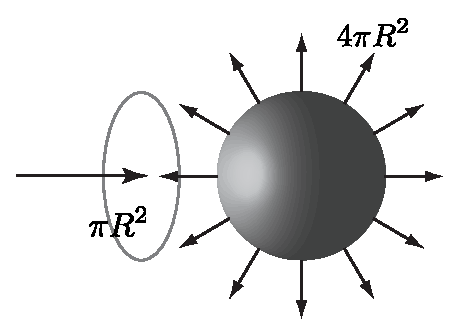
\includegraphics[width=\linewidth]{fig/io.eps}
\end{center}
	\caption{惑星へ入射してくる恒星光と惑星表面から出ていく輻射光。}
	\label{fig:io}
\end{figure} 

半径$R$の惑星が受け取るエネルギーは、恒星フラックス密度 \index{こうせいふらっくすみつど@恒星フラックス密度} (stellar flux density) $S$を用いて
\begin{align}
\label{eq:lab}
L_{\mathrm{ab}}=(1-A) \pi R^2 S  
\end{align}
と書くことができる。$\pi R^2$は惑星の断面積である(図\ref{fig:io}参照)。$A$は惑星全体の反射率(アルベド\index{アルベド@アルベド}という)で$(1-A)$の項は反射して宇宙に返された分を除いている。恒星光を黒体輻射と考えると、恒星フラックス密度は
\begin{align}
  \label{eq:starfluxdens}
S= \frac{L_\star}{4 \pi a^2} = \frac{4 \pi R_\star^2 \sigma T_\star^4}{4 \pi a^2}\,\,\mathrm{[W/m^2]} 
\end{align}
である。$a$は公転半径、$R_\star$は恒星半径、$T_\star$は恒星温度、$\sigma$はシュテファンボルツマン定数である。地球における$S_\odot =1370 \mathrm{W/m^2}$は太陽定数\index{たいようていすう@太陽定数}とよばれる。
一方、惑星からの放射を温度$T_{\mathrm{eq}}$の黒体輻射とすると放射エネルギーは
\begin{align}
\label{eq:lem}
L_{\mathrm{em}} = \beta ( 4 \pi R^2 \sigma T_{\mathrm{eq}}^4 ) + L_\mathrm{int}
\end{align}
とかける。ここで$ L_\mathrm{int}$は惑星自身のエネルギー放射である。若い惑星ではこの項が卓越しているため自己放射惑星と呼ばれる。

$\beta$は熱分配の度合いを表す係数で、瞬時に全球に一様に分配する極限$\beta=1$と、恒星光のあたっている半球だけに分配される場合$\beta=0.5$の間の値をとる。潮汐力により公転と自転が一致(潮汐ロック)しているような恒星に近い惑星では、地球に対する月のように、惑星の同じ面が常に恒星方向を向くために導入される補正である。


通常のmatureな惑星の場合、自己放射が無視できるため$L_\mathrm{int}=0$とおける。この場合、恒星からの吸収エネルギーが輻射エネルギーと釣り合うはずである。
\begin{align}
\label{eq:lemeqi}
  L_{\mathrm{em}} = L_{\mathrm{ab}}
\end{align}
とした時(放射平衡)の$T_{\mathrm{eq}}$を放射平衡温度\index{ほうしゃへいこうおんど@放射平衡温度}(単に平衡温度ともいう)と呼ぶ。この時、式(\ref{eq:lab})から式(\ref{eq:lemeqi})までを用いると
\begin{align}
  \label{eq:eqteq}
 \frac{T_{\mathrm{eq}}^4 a^2 }{T_\star^4 R_\star^2} = \frac{1-A}{4 \beta}
\end{align}
となる。つまり
\begin{align}
 T_\mathrm{eq} &= \left(\frac{1-A}{4 \beta}\right)^{\frac{1}{4}} T_\star \sqrt{\frac{R_\star}{a}} \\
&= 396 \mathrm{K}  \left(\frac{1-A}{4 \beta}\right)^{\frac{1}{4}} \left( \frac{T_\star}{5800 \mathrm{K}}\right) \left( \frac{R_\star}{R_\odot}\right)^{\frac{1}{2}} \left( \frac{a}{1 \mathrm{au}}\right)^{-\frac{1}{2}} \\
&= 396 \mathrm{K}  \left(\frac{1-A}{4 \beta}\right)^{\frac{1}{4}} \left( \frac{L_\star}{L_\odot}\right)^{\frac{1}{4}} \left( \frac{a}{1 \mathrm{au}}\right)^{-\frac{1}{2}}
\end{align}
となる。

ここで惑星表面が受け取る平均的な恒星フラックスを定義しておこう。式(\ref{eq:lab})より
\begin{align}
\label{eq:aveinpuF}
  F_\star &\equiv \frac{L_{\mathrm{ab}}}{4 \pi R^2}= \frac{(1 - A)}{4} S \\
  &= 240 \left(\frac{1-A}{0.7}\right) \left(\frac{S}{S_\odot}\right) \mathrm{W/m^2} 
\end{align}
のように$S$と結びつく。この式は、恒星の入射エネルギーから惑星の反射分を取り除き、図\ref{fig:io}に示すような断面円で入ってきた入射フラックスが自転により球面へ分配される効果を表す係数$1/4$をかけたものになるという描像を表している。惑星が受け取る平均フラックス密度と放射平衡温度には、
\begin{align}
  \label{eq:teq}
\sigma T^4_{\mathrm{eq}} = F_\star/\beta 
\end{align}
の関係にあることもわかる。

\subsection*{Radiance, Irradiance}

惑星や恒星は遠方から見れば点であり、近づいてみれば通常、連続的に密度が変わる三次元構造を持っている。しかし表面上のある基準球面、たとえば地球なら惑星表面や大気上端の高度一定面、恒星なら光球面などを考えると、ある面からの放射や、ある面への放射を考える事で、計算が易しくなる。そこで、まず、ある有限面積の表面からの放射や、表面への放射を定量化するための量を定義しよう。微小面積$d A$からある${\bf \Omega}$方向に$d \Omega$のコーン内(図\ref{fig:int}左)を通過する単位時間・単位波長あたりのエネルギー$d E$を考える。${\bf n}$は単位法線ベクトルである。$d E$自体は、見かけの投影面積$\cos{\theta} d A$に比例するので、
\begin{align}
d E = L_{\uparrow}(\theta,\phi) \cos{\theta} d A d \Omega d \nu
\end{align}
のように比例定数を、radiance (放射輝度) \index{Radiance@Radiance} $L_{\uparrow}$として定義すれば、投影の効果を除いて放射を定義できる。単位は例えば[$\mathrm{W/m^2/sr/\mu m}$]となる。$dA$から${\bf n}$方向に流れるネットのエネルギーをirradiance (放射照度) \index{Irradiance@Irradiance} $E_{\uparrow}$といい
\begin{align}
E_{\uparrow} &= \int_{\mathrm{us}} d E = \int  d \Omega L_{\uparrow} (\theta,\phi) \cos{\theta} \\
\label{eq:rad}
&= \int_{0}^{2 \pi} d \phi  \int_{0}^{\pi/2} d \theta L_{\uparrow} (\theta,\phi) \cos{\theta} \sin{\theta}
\end{align}
となる。usは上半球面の意味である。

\begin{figure}[]
 \begin{center}
	\includegraphics[width=\linewidth]{fig/radiance_bw.png}
	\includegraphics[width=\linewidth]{fig/brdfdef_bw.png}
\end{center}
	\caption{(上)素片$d A$からの放射または、素片への放射。(下)($\vartheta_0,\varphi_0$)方向からの平行光の入射と立体角$d \Omega$あたりの($\vartheta_0,\varphi_0$)方向への反射。}
	\label{fig:int}
\end{figure} 

\section{輻射スペクトル}

半径$R_p$で温度$T$の球から発する黒体輻射を距離$d$で測定した時のフラックスを考える。
温度$T$を持った表面は黒体輻射を行う。黒体輻射のRadianceは
\begin{align}
L_{\uparrow} d \lambda = B_\lambda (T) d \lambda = \frac{2 h c^2}{\lambda^5} \frac{1}{\exp{(hc/\lambda k_B T)}-1} d \lambda
\end{align}
でである。素片$d A$から$d \Omega$の放射コーンを考え、距離$d$にある面積$d A_\mathrm{tel}$の望遠鏡がコーンの先端と考える($d \Omega = d A_\mathrm{tel}/d^2$)と、$d A$から$d A_\mathrm{tel}$が受け取るエネルギー$\Delta E d A_\mathrm{tel}$は、
\begin{eqnarray}
\label{eq:brdfdef3}
\Delta E d A_\mathrm{tel} &=& L_\uparrow \cos{\vartheta_1} d \Omega d A \\
&=& \frac{L_\uparrow}{d^2} \cos{\vartheta_1} d A d A_\mathrm{tel}
\end{eqnarray}
となる。すなわち、観測者から見た素片$d A$によるIrradianceもしくはフラックスは
\begin{eqnarray}
\label{eq:brdfdef6}
\Delta E = \frac{L_\uparrow}{d^2} \cos{\vartheta_1} d A
\end{eqnarray}
となる。

これを全球で積分して、
\begin{align}
\label{eq:raddef}
f_p &= \int_\mathrm{planet} \Delta E = \int_\mathrm{planet} d A \frac{B_\nu (T)}{d^2} \cos{\vartheta_1} \\
&= R_p^2 B_\nu (T) \int_0^{2 \pi} d \varphi_1 \int_0^{\pi/2} d \vartheta_1 \sin{\vartheta_1} \cos{\vartheta_1}\\
&= \pi B_\nu (T) \frac{R_p^2}{d^2}
\end{align}
となる。全エネルギーは波長方向の積分と距離$d$の球殻面積をかけて
\begin{align}
\label{eq:raddeftot}
L &= 4 \pi d^2 \int_0^{\infty} d \nu \pi B_\nu (T) \frac{R_p^2}{d^2} = 4 \pi R_p^2 \sigma T^4  
\end{align}
となる。\\


惑星からの輻射スペクトルは第ゼロ近似では、単一温度$T_p$の黒体輻射
\begin{align}
f_p (\lambda) d\, \lambda  &= \pi B_\lambda(\lambda,T_p) \frac{ R_p^2}{d^2}  d \lambda \\
&= \frac{2 \pi h c^2}{\lambda^5} \frac{ R_p^2}{d^2} \left[ \exp{ \left(\frac{h c}{\lambda k_B T_p} \right) }- 1 \right]^{-1} d\, \lambda ,
\label{eq:planckdist}
\end{align}
で近似することができる場合がある。

例えば、ほぼ大気の存在しない地球の輻射スペクトルは、表面温度の$T=200--300$Kの黒体輻射でおおまかに近似できる。しかし、ガス惑星や褐色矮星に関しては、黒体輻射の近似はあまりよくない。これは大気中の分子の強い吸収によるところが大きい。放射スペクトルは、大気中の光学的厚さが1付近になる深さの大気層の黒体輻射に近い光によるが、これは大気中の分子により波長ごとに大きく変化する。この黒体輻射からの大きな破れが、系外惑星大気の特徴である。\\


\begin{itembox}{上向き射出フラックス}
\footnotesize
\color{gray}
大気の放射平衡モデルでは、大気高さ方向の一次元モデルのフラックスを考えるが、境界条件に地表のフラックスを与えることがある。同様にある黒体放射の素片から上向き射出されるフラックスを考えよう。素片周囲の上半面での角度積分を考えて
\begin{align}
\label{eq:defsurf}
F_\nu (T) &= \Delta E = \int_\mathrm{us} d \Omega B_\nu (T) \cos{\vartheta_1} = \pi B_\nu (T)
\end{align}
となる。全エネルギーでは同様に波長積分をして
\begin{align}
\label{eq:defsurflum}
F (T) &= \int d \nu f_\nu (T) = \sigma T^4 
\end{align}
となる。
\end{itembox}

\section{反射・散乱スペクトル}

反射光は、反射面・観測者との相対位置により観測される強度がことなるので若干複雑である。しかし平均的には以下のように考えることができる。まず、式(\ref{eq:lab})の時に、惑星が受け取らなかったエネルギーが反射となるので、反射のエネルギーは
\begin{align}
    L^\mathrm{ref}_p = A \pi R_p^2 S = \frac{L_\star}{4 \pi a^2} \pi R_p^2 A
\end{align}
である。距離$d$で受け取る反射フラックスは平均的には
\begin{align}
    \langle f_{p}^\mathrm{ref} \rangle = \frac{ L^\mathrm{ref}_p}{4 \pi d^2}
\end{align}
であるから、恒星のフラックス
\begin{align}
    f_\star = \frac{L_\star}{4 \pi d^2}
\end{align}
を用いて、
\begin{align}
    \langle f_{p}^\mathrm{ref} \rangle = \frac{A}{4} \left( \frac{R_p}{a} \right)^2 f_\star
\end{align}
となる。

スペクトルの観点からは、波長の関数となっているのは$A$と$f_\star$の掛け算、つまり恒星スペクトルに反射スペクトルがかかったものであるという点である。
\begin{align}
    \langle f_{p}^\mathrm{ref} \rangle (\lambda) d \lambda = \frac{1}{4} \left( \frac{R_p}{a} \right)^2 A(\lambda) f_\star (\lambda) d \lambda
\end{align}
である。

平均ではなく位相の関数としてフラックスを求めるのは少し複雑であるのでここでは割愛する。詳しくは拙著、系外惑星探査5.1.1を参照のこと。ここでは結果だけ紹介する。距離$d$の位置から観測した惑星の反射光フラックス$f_p^\mathrm{ref} (\lambda)$は、主星-惑星間距離$a$, 惑星アルベド$A(\lambda)$、惑星半径$R_p$、距離$d$から観測した主星フラックス$f_\star (\lambda)$、また観測者から見た惑星位置による関数$\phi (\beta)$を用いて
\begin{align}
\label{eq:refplanet}
f_p^\mathrm{ref} (\lambda) = \frac{2 \phi(\beta)}{3} A(\lambda) \left(\frac{R_p}{a}\right)^2 f_\star (\lambda),
\end{align}
\begin{align}
\label{eq:phaselambert}
\phi(\beta) \equiv [\sin{\beta} +  (\pi - \beta) \cos{\beta}]/\pi, 
\end{align}
と表される。ここで$\phi (\beta)$はLambert phase function\index{Lambert phase function@Lambert phase function}とよばれ、位相角(phase angle) $\beta = \angle $(主星ー惑星ー観測者)の関数である。ただしこの関係は、等方散乱を仮定していることに注意が必要である。海洋による鏡面反射(ocean glint)などの非等方性の強い反射では必ずしも成り立たない。

恒星光が惑星にあたって反射・散乱する光は、現在の技術では、宇宙からの精密測光での位相カーブとしての検出などの限定された条件でしか達成されていないが、原理的には惑星表面の二次元分布情報を持つ豊かな情報源である。反射光で重要な指標は主星と惑星のフラックス比、{\bf 主星惑星コントラスト}\index{しゅせいわくせいこんとらすと@主星惑星コントラスト}
\begin{align}
\label{eq:contrast}
c_{\mathrm{sp}} (\lambda) \equiv \frac{f_p (\lambda)}{f_\star (\lambda)}
\end{align}
である。主星惑星コントラストが緩いほうが直接撮像においても位相カーブにおいても検出が容易となる。

半月ならぬ半惑星($\beta=90^\circ$)の場合、式(\ref{eq:refplanet})を用いて、主星惑星コントラストを見積もることができる。地球の場合
\begin{align}
\label{eq:refplanetearth}
c_\mathrm{sp}  \approx 10^{-10} \left( \frac{A}{0.3} \right) \left(\frac{R_p}{R_\oplus} \right)^{2} \left(\frac{a}{1 \, \mathrm{au}} \right)^{-2}
\end{align}
程度に、ホットジュピターの場合
\begin{align}
\label{eq:refplanetearth}
c_\mathrm{sp}  \approx 10^{-6} \left( \frac{A}{0.1} \right) \left(\frac{R_p}{R_J} \right)^{2} \left(\frac{a}{0.05 \, \mathrm{au}} \right)^{-2}
\end{align}
程度になることがわかる。

